\documentclass[xcolor={usenames,dvipsnames}]{beamer}

\mode<presentation> { }

\usetheme{metropolis}
\usepackage{listings}
\usepackage{polyglossia}
\setmainlanguage{english}


\usepackage[numbers]{natbib}

\usepackage{tikz}
\usetikzlibrary{arrows, decorations.pathmorphing,backgrounds,fit,positioning,shapes.symbols,chains, positioning,automata}

\usepackage{lstc}
\usepackage{lstnasm}
\usepackage{lstshell}
\renewcommand{\lstcurrentinputdir}{listings}
\usepackage{multirow}

\usepackage{tikz}
\usetikzlibrary{arrows,
decorations.pathmorphing,backgrounds,fit,positioning,shapes.symbols,chains,
positioning,automata,positioning,calc}

\tikzset{onslide/.code args={<#1>#2}{%
  \only<#1>{\pgfkeysalso{#2}} % \pgfkeysalso doesn't change the path
}}

\makeatletter
\newenvironment<>{btHighlight}[1][]
{\begin{onlyenv}#2\begingroup\tikzset{bt@Highlight@par/.style={#1}}\begin{lrbox}{\@tempboxa}}
{\end{lrbox}\bt@HL@box[bt@Highlight@par]{\@tempboxa}\endgroup\end{onlyenv}}

\newcommand<>\btHL[1][]{%
  \only#2{\begin{btHighlight}[#1]\bgroup\aftergroup\bt@HL@endenv}%
}


\def\bt@HL@endenv{%
  \end{btHighlight}%   
  \egroup
}

\newcommand{\bt@HL@box}[2][]{%
  \tikz[#1]{%
    \pgfpathrectangle{\pgfpoint{1pt}{0pt}}{\pgfpoint{\wd #2}{\ht #2}}%
    \pgfusepath{use as bounding box}%
    \node[anchor=base west, fill=orange!30,outer sep=0pt,inner xsep=1pt, inner ysep=0pt, rounded corners=3pt, minimum height=\ht\strutbox+1pt,#1]{\raisebox{1pt}{\strut}\strut\usebox{#2}};
  }%
}

\makeatother



%settings 
\everymath{\displaystyle}

\title{Dynamic libraries explained }
\subtitle{as seen by a low-level programmer}
\author{I.Zhirkov}

\date{2017}
\AtBeginSection[]{
  \begin{frame}
  \vfill
  \centering
  \begin{beamercolorbox}[sep=8pt,center,shadow=false,rounded=false]{title}
    \usebeamerfont{title}\insertsectionhead\par%
  \end{beamercolorbox}
  \vfill
  \end{frame}

%\begin{frame}
%    \tableofcontents[currentsubsection,
%      subsectionstyle=show/hide/show, sectionstyle=hide/hide]
%\end{frame}
}


%\AtBeginSection[]
%{
%  \begin{frame}<beamer>{\secname}
%    \tableofcontents[currentsection, currentsubsection,
%      subsectionstyle=show/show/hide, sectionstyle=show/show]
%  \end{frame}
%}



\begin{document}

\begin{frame}
  \titlepage
\end{frame}


\begin{frame}{Exemplary environment}
    \begin{itemize} 
        \item  Intel 64 aka AMD64 aka x86\_64.
        \item  GNU/Linux
        \item  Object file format: ELF files.
        \item Languages: C, Assembly (NASM)
\end{itemize} 
\end{frame}


\begin{frame}{Sources}

    \begin{itemize}
        \item ELF format specification  
        \item System V Application Binary Interface
        \item U.Drepper -- ``How to write shared libraries''

        \item \url{http://amir.rachum.com/blog/2016/09/17/shared-libraries/}
        \item I.Zhirkov -- ``Low-level programming: C, Assembly and Program Execution''
\end{itemize} 

\end{frame}
\begin{frame}{Contents}
    \tableofcontents[subsectionstyle=hide/hide/hide]
\end{frame}

\section{Prerequisites}

\begin{frame}[fragile]{Assembly (NASM)} 
    \begin{itemize}
        \item  Registers:  \asm{rax, rbx, rcx,...}; \asm{rip}
        \item  Sections: code (.text) separated from data (.data)
        \item  \sh{label: instruction ; comment}
        \item  Addressing modes:
        \item  \asm{ db 1} | \asm{ dw 2}|  \asm{ dd 4} | \asm{ dq 8} 
\begin{asmexample}
    var: dq 42, 43, 44
    mov rax, 42             ; imm
    mov rax, var            ; address
    mov rax, [var]          ; value (42)
    mov rax, [var + 8]      ; value (43)
    mov rax, [var + 8*rcx]  ; value (43)
\end{asmexample}
\end{itemize} 
\end{frame}
\section{Preface}
\subsection{Relocation}

\begin{frame}{\subsecname}
    \begin{itemize}
 \item  Compiling is not trivial.  

 \item  We have Random Access Memory, linear addresses.  

 \item  Challenge: carefully placing code and data in memory.

\end{itemize} 
\end{frame}

\begin{frame}[fragile]{Example}

    \begin{tabular}{p{5.3cm} l}
        {
        
\begin{cexample}
int x;
int* y = &x;

void f() {
    x = x + 1;
}
\end{cexample}


        \only<2>{
       
\begin{itemize}
    \item  Where to place \c{x} and \c{y}?
    \item  Code and data require knowing addresses. 
    \item  \emph{Once an address is picked, it is difficult to change.}
\end{itemize}

        }

        }&{
            \raisebox{-\height}{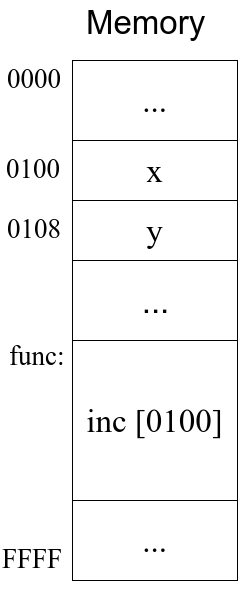
\includegraphics[scale=0.3]{images/relocation-1.png}

       ~

       ~

        }


        }
        \\
        & 
        \only<1>{\small{ {\color{red} red} -- depends on positioning}} 
    \end{tabular}

\end{frame}



\begin{frame}{Solution: linking stage}
    \begin{itemize}

        \item Last stage of compilation: linking.
        \item  Defer placement until linking.
            \begin{itemize}
                \item  Instructions generated, we know all functions and global variables.
            \end{itemize} 
        \item  \textbf{Symbol} -- program entities which are useful for linking.
            \begin{itemize}
                \item Anything with an absolute address 
                    \begin{itemize}

                        \item Global variables.
                        \item Functions.
                    \end{itemize}
                \item Utility symbols.
            \end{itemize} 
\end{itemize} 
    
    

\end{frame}



\begin{frame}[fragile]{Symbols}

For each symbol we know its:
    \begin{itemize}
        \item  Name.
        \item  Address (if assigned).
        \item  Locations where referenced.
\end{itemize} 
     Assigning addresses to symbols is called \textbf{relocation}.

\begin{cexample}
int x;          // symbol 'x'

void func() {   // symbol 'f'
    x = x + 1;  // symbol 'x' referenced
}
\end{cexample}


\end{frame}

\subsection{Linker}
\begin{frame}{\subsecname}
    
    \textbf{Linker} is a program that assigns addresses to symbols and finalizes
    compilation.
    
    Allows for separate compilation, which we need:
    
    \begin{itemize}
        \item Programs too big for one file (split into modules).
        \item Using already compiled code (libraries).
        \item Fast debugging (each change invokes recompilation).
            \begin{itemize}
                \item  Some programs take \emph{hours} to compile from scratch.
            \end{itemize}
    \end{itemize} 

\end{frame}



\begin{frame}{Compilation pipeline}
    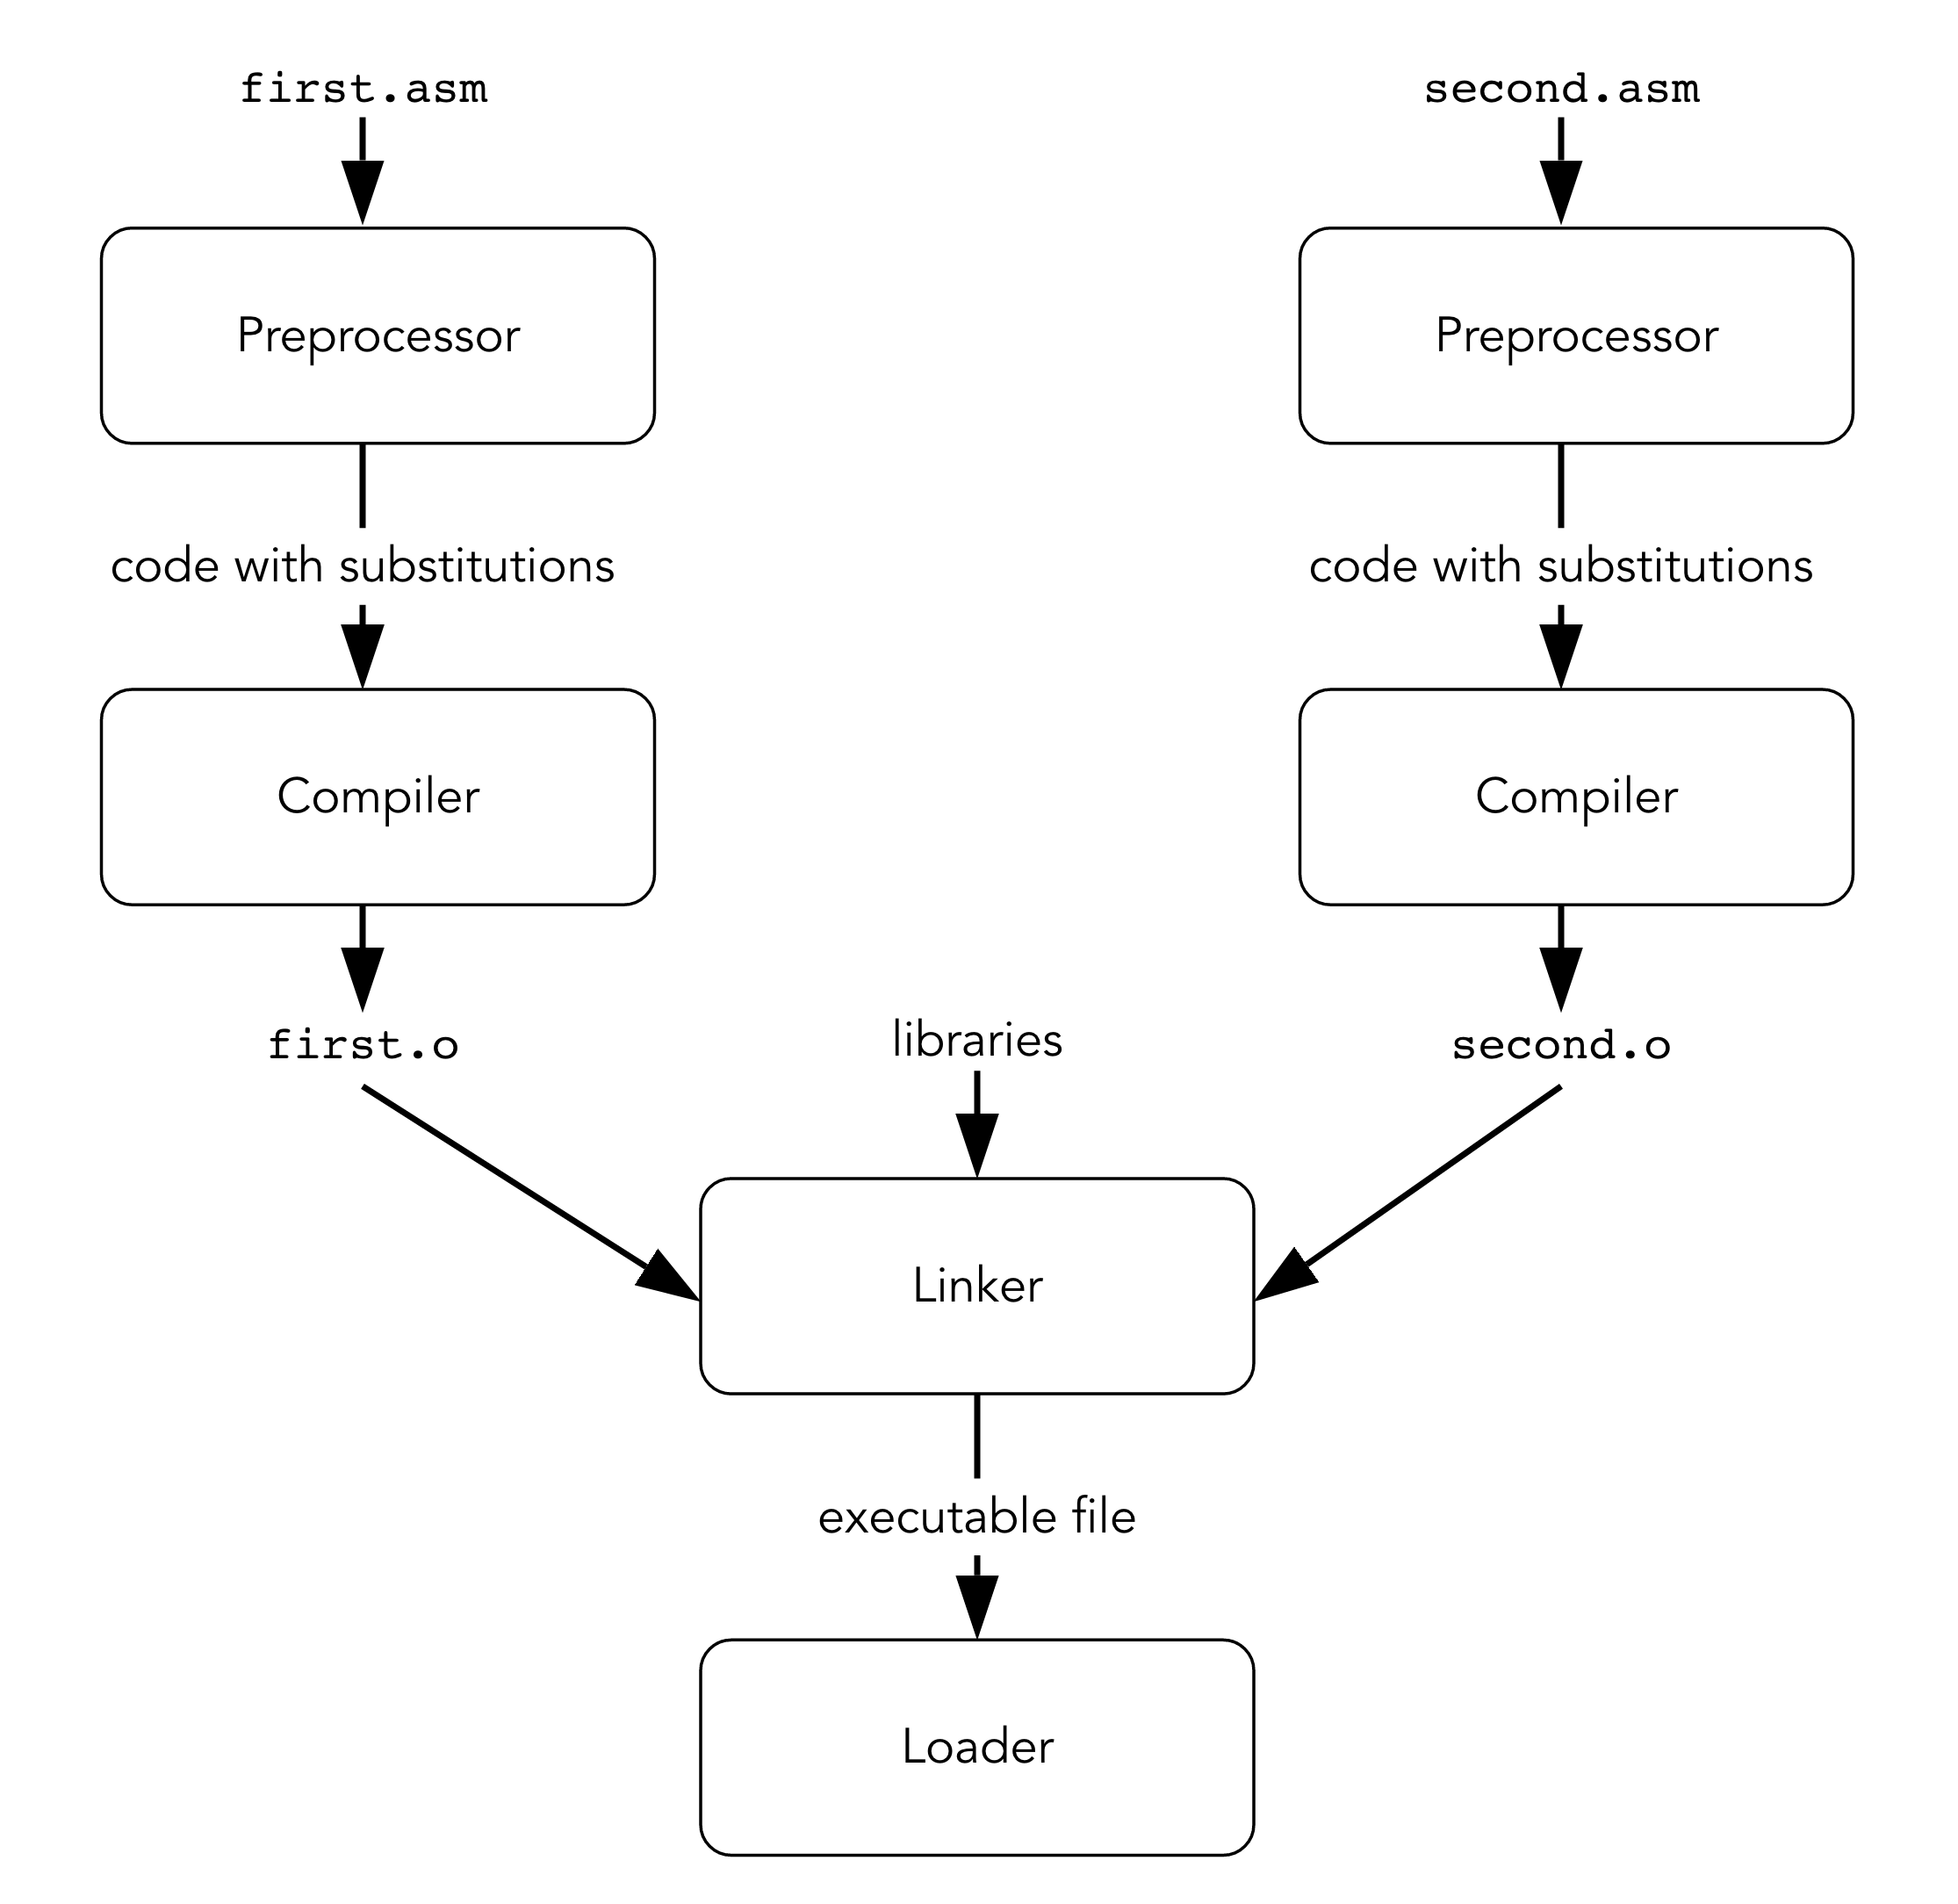
\includegraphics[height=\textheight]{images/compilation.png} 
\end{frame}


\begin{frame}[fragile]{Modules and objects}
    Compiler works with atomic code entities called \textbf{modules}.
   
    In C and assembly, a module corresponds to a  \sh{.c} or \sh{.asm} file.
    
    Modules are transformed into \textbf{object files}.
    
Object files are structured and contain translated instructions.


\end{frame}

\begin{frame}{ELF object files}
\textbf{ELF} -- Executable and Linkable Format, typical for *nix systems.

Can be:

\begin{enumerate}
\item \textbf{Relocatable} 
    
    {\small \texttt{.o}-files, produced by compiler, not linked.}

    {\small Same as \textbf{static libraries}}.

\item \textbf{Executable} 
    
    {\small program after linking, ready-to-run.}

\item \textbf{Shared} 
   
    {\small \texttt{.so}, dynamic libraries, to be linked in runtime.}

\end{enumerate}

    \begin{description}
        \item[Static linker] transforms 1 into 2 or 3.
        \item[Dynamic linker] prepares 3 for execution.
    \end{description}

\end{frame}


\section{Static linking}

\subsection{ELF overview}


\begin{frame}{Toolset}
    Tools to examine object files:
    \begin{itemize}
\item  \sh{readelf} -- ELF meta-information 
\item  \sh{objdump} -- meta-information of any format, disassembler
\item  \sh{nm} -- only symbols.
\end{itemize} 

What we use:
    \begin{itemize}
        \item  \sh{objdump} usually, less specific
        \item \sh{readelf} for verbose ELF structure
    \end{itemize} 

\end{frame}

\begin{frame}{ELF file structure}
        Three headers:
        \begin{itemize}
            \item  File header 
                \begin{itemize}
                    \item  General info.
                    \item  Links to Program and Section headers.
                \end{itemize} 
            \item  Section header
                \begin{itemize}
                    \item Information about \textbf{sections}.
                    \item Each section stores code or meta-information.
                    \item Needed for linking.
                \end{itemize} 
            \item  Program header
                \begin{itemize}
                    \item  Instructions on how to create process image.
                    \item  Information about \textbf{segments}.
                    \item  Segment is a virtual memory region;
                        contains some sections.

                    \item Needed for execution.
                \end{itemize} 
        \end{itemize} 

        {\small \textbf{Memory region} -- consecutive memory pages with same permissions.}
\end{frame}


\begin{frame}[fragile]
    \begin{tabular}{p{5cm} p{5cm}}
       
            
            \raisebox{-\height}{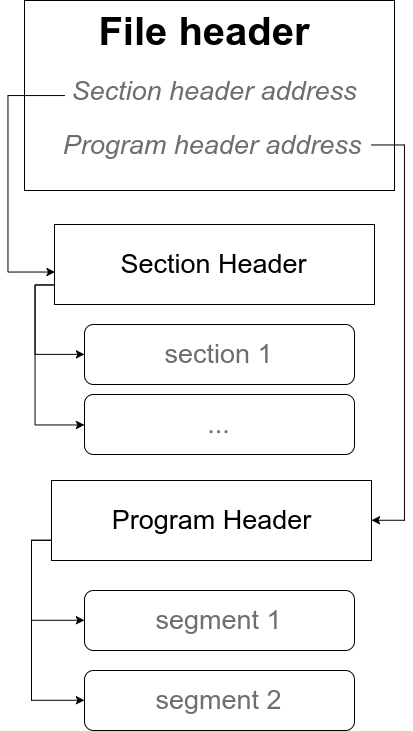
\includegraphics[scale=0.3]{images/elf-structure-general.png}}
            
        & {
            ~

Typical sections:
            
            \begin{itemize}
                \item \textbf{.data}
                \item \textbf{.text} -- compiled instructions.
                \item \textbf{.rodata} -- read only.
                \item \textbf{.bss} -- zero-initialized data (only size is stored).
                \item \textbf{.line} -- line numbers in source code.
                \item \textbf{.symtab} -- symbol table.  
                \item \dots
            \end{itemize} 

        }
    \end{tabular}
\end{frame}

\begin{frame}[fragile]{Exemplary program}
  
    \begin{asmexample}
section .data         ; global variables:
x: dq 148842          ; int  x = 148842
y: dq x               ; int* y = &x

extern somewhere      ; an external symbol 
global _start         ; visible to other modules

section .text         ; code:  {
  _start: 
    mov rax, x        ; rax := &x
    mov rdx, y        ; rdx := &y

  jmp _start          ; } while (true);
    \end{asmexample}

\end{frame}


\begin{frame}[fragile]{ELF File Header}

    \begin{shell}
> nasm -f elf64 -o symb.o symb.asm  # compile 
> ld -o symb symb.o                 # link
> readelf -h  symb             # view file header
    \end{shell}

Class:                             ELF64

Type:                              EXEC (Executable file)

Entry point address:               0x4000c0

Start of program headers:          56 (bytes into file)

Start of section headers:          584 (bytes into file)

Number of program headers:         2

Number of section headers:         6
\end{frame}

\subsection{Sections in relocatable file}

\begin{frame}[fragile]{Sections -- before linking}
    \begin{shell}
> objdump -h symb.o
    \end{shell}

{
%\setlength{\parindent}{-0.5cm}
\setlength{\tabcolsep}{12pt}

    \begin{tabular}{l  l  l  l  l  l }
        \textbf{No}  &  \textbf{Name} & \textbf{Size} & \textbf{Address} & \textbf{Offset} & \textbf{Align} \\\hline
        1 & .data  &      0x10 & 0& 0x240 & 4 \\
        \multicolumn{6}{r}{\small \textsc{ contents, alloc, load, reloc, data}} \\
\hline
        2 & .text &      0x16& 0& 0x250 & 16 \\
        \multicolumn{6}{r}{\small \textsc{contents, alloc, load, reloc, readonly, code}}\\
\hline
    \end{tabular} 
}
\pause
    \begin{itemize}
        \item Stubs for addresses.
        \item Offset from file start.
        \item \texttt{objdump} omits excess information.
    \end{itemize}
\end{frame}

\begin{frame}[fragile]{Sections -- before linking}

    \sh{readelf} is more verbose.

    \begin{shell}
> readelf -S symb.o
    \end{shell}

{\small
\setlength{\parindent}{-0.5cm}
\setlength{\tabcolsep}{3pt}
\begin{tabular}{l l l l l l l l l l }
\textbf{Name}& \textbf{Type} & \textbf{Address} & \textbf{Offset} & \textbf{Size}& \textbf{EntSize} & \textbf{Flags} & \textbf{Link} & \textbf{Info} & \textbf{Align} \\
\hline
.data & PROGBITS   & 0 & 240  & 10 & 0 & WA & 0 & 0 & 4 \\
.text & PROGBITS   & 0 & 250  & 16 & 0 & AX & 0 & 0 & 16 \\
.shstrtab & STRTAB & 0 & 270  & 3d & 0 & 0  & 0 & 0 & 1  \\
.symtab   & SYMTAB & 0 & 2b   & c0 & 18& 0  & 5 & 6 & 4  \\
.strtab   & STRTAB & 0 & 370  & 2d & 0 & 0  & 0 & 0 & 1  \\
.rela.data& RELA   & 0 & 3a0  & 18 & 18& 0  & 4 & 1 & 4 \\
.rela.text& RELA   & 0 & 3c0  & 30 & 18& 0  & 4 & 2 & 4 \\
\hline
\end{tabular}
}

    \sh{.symtab} stores the symbol table.
    
    \sh{.rela.<section-name>} store relocations.
\end{frame}


\begin{frame}[fragile]{Symbol table before linking}
  

\begin{shell}
> objdump -tf symb.o 
start address 0x0
\end{shell}

{
\setlength{\tabcolsep}{10pt}
    \begin{tabular}{l l l l}

\textbf{Address}& \textbf{Type} & \textbf{Section} & \textbf{Name} \\
\hline
    0x0 &  \texttt{l    df} & *ABS*  &  symb.asm\\
    0x0 &  \texttt{l    d } & .data  &  .data\\
    0x0 &  \texttt{l    d } & .text  & .text\\
    0x0 &  \texttt{l      } & .data  &  x\\
    0x8 &  \texttt{l      } & .data  &  y\\
    0x0 &  \texttt{       } & *UND*  &  somewhere\\
    0x0 &  \texttt{g      } & .text  & \_start\\
\hline
\end{tabular}

}
\begin{itemize}
\item[\texttt{l}] --  local

\item[\texttt{g}] --  global (visible to other object files)

\item[\texttt{d}] --  debug symbol

\item[\texttt{f}] --  file name  

\end{itemize}

\end{frame}


\begin{frame}{Symbol table before linking}
    \begin{itemize}

        \item  Addresses are relative to section starts
        \item  Utility symbols are marked as debug
        \item  External symbols are in \textsc{*UND*} section
        \item  \textsc{*ABS*} as ``unrelated to sections''.

\end{itemize} 
\end{frame}


\begin{frame}[fragile]{Stubs are also in code}
    
    {\usebeamerfont{title} Source }

\begin{asmexample}
  _start: 
    mov rax, x        
    mov rdx, y        
  jmp _start          
\end{asmexample}

    {\usebeamerfont{title} Disassembly }
\begin{shell}
> objdump -d -mintel-mnemonic symb.o
\end{shell}

\begin{asmexample}
0000000000000000 <_start>:
   0:   48 b8 @00 00 00 00 00@    mov rax, @0x0@
   7:   @00 00 00@ 
   a:   48 ba @00 00 00 00 00@    mov rdx, @0x0@
  11:   @00 00 00@ 
\end{asmexample}

\end{frame}


\begin{frame}[fragile]{Relocations}
    \begin{itemize}
        \item  We need to keep track of the stubs.
        \item  Sections of interest: \textbf{.data}, \textbf{.rodata}, \textbf{.text}.
    \end{itemize} 


\begin{shell}
> objdump -r symb.o
\end{shell}

    \begin{tabular}{p{7cm} l }
        {
Relocations in .data:

    \begin{tabular}{ l l l }
        \textbf{Offset} & \textbf{Type} & \textbf{Value} \\
        \hline
        0x8 & \texttt{R\_X86\_64\_64} & .data \\
        \hline
    \end{tabular}

} & {

\begin{asmexample}


x: dq 148842 
y: dq x
\end{asmexample}
        } \\
        {
Relocations in .text:

    \begin{tabular}{ l l l }
        \textbf{Offset} & \textbf{Type} & \textbf{Value} \\
        \hline
        0x2 & \texttt{R\_X86\_64\_64} & .data \\
        0xc & \texttt{R\_X86\_64\_64} & .data+0x8 \\
        \hline
    \end{tabular}
}
        & {

\begin{asmexample}


mov rax, x
mov rdx, y
\end{asmexample}



        }
    \end{tabular}

\end{frame}

\subsection{Sections in linked file}

\begin{frame}[fragile]{\subsecname}
    
\begin{shell}
> ld -o symb symb.o
\end{shell}
    
{
\setlength{\tabcolsep}{12pt}

    \begin{tabular}{l  l  l  l  l  l }
        \textbf{No}  &  \textbf{Name} & \textbf{Size} & \textbf{Address} & \textbf{Offset} & \textbf{Align} \\\hline
        1 & .text &      0x16& 0x4000b0 & 0xb0 & 16 \\
        \multicolumn{6}{r}{\small \textsc{contents, alloc, load, readonly, code}}\\
\hline
        2 & .data  &      0x10 & 0x6000c8& 0xc8 & 4 \\
        \multicolumn{6}{r}{\small \textsc{ contents, alloc, load, data}} \\
\hline
    \end{tabular} 
}
\pause
    \begin{itemize}
        \item Addresses are chosen.
        \item No more \textsc{reloc} mark.

    \end{itemize}
    
\end{frame}


\begin{frame}[fragile]{Symbol table after linkage}
  

\begin{shell}
> objdump -tf symb
Flags: EXEC_P, HAS_SYMS, D_PAGED
start address 0x4000b0
\end{shell}

{
\setlength{\tabcolsep}{10pt}
    \begin{tabular}{l l l l}

\textbf{Address}& \textbf{Type} & \textbf{Section} & \textbf{Name} \\
\hline
0x4000b0 & \texttt{ l    d } & .text &	 .text     \\
0x6000c8 & \texttt{ l    d } & .data &	 .data     \\
0x000000 & \texttt{ l    df} & *ABS* &	 symb.asm  \\
0x6000c8 & \texttt{ l      } & .data &	 x         \\
0x6000d0 & \texttt{ l      } & .data &	 y         \\
0x000000 & \texttt{        } & *UND* &	 somewhere \\
0x4000b0 & \texttt{ g      } & .text &   \_start    \\
0x6000d8 & \texttt{ g      } & .data &	 \_\_bss\_start\\
0x6000d8 & \texttt{ g      } & .data &	 \_edata    \\
0x6000d8 & \texttt{ g      } & .data &	 \_end      \\
        \hline
\end{tabular}

}

\begin{itemize}
\item[\texttt{l}] --  local

\item[\texttt{g}] --  global (visible to other object files)

\item[\texttt{d}] --  debug symbol

\item[\texttt{f}] --  file name  

\end{itemize}

\end{frame}


\subsection{Program Headers}

\begin{frame}{\subsecname}
    \begin{itemize}
\item  Created after static linking (shared / executable object files).
\item  Each entry is a segment or other information for execution.
    \end{itemize} 

\end{frame}

\begin{frame}{Segments}
    \textbf{Confusion: everything is called ``segment''}
    \begin{itemize}
        \item  Real/Protected mode segments.
        \item  ELF segments
        \item ``Segmentation fault''
        \item  ... 
    \end{itemize} 

    ELF segment maps some sections to a region of memory.
\end{frame}

\begin{frame}{Mapping sections into memory}
    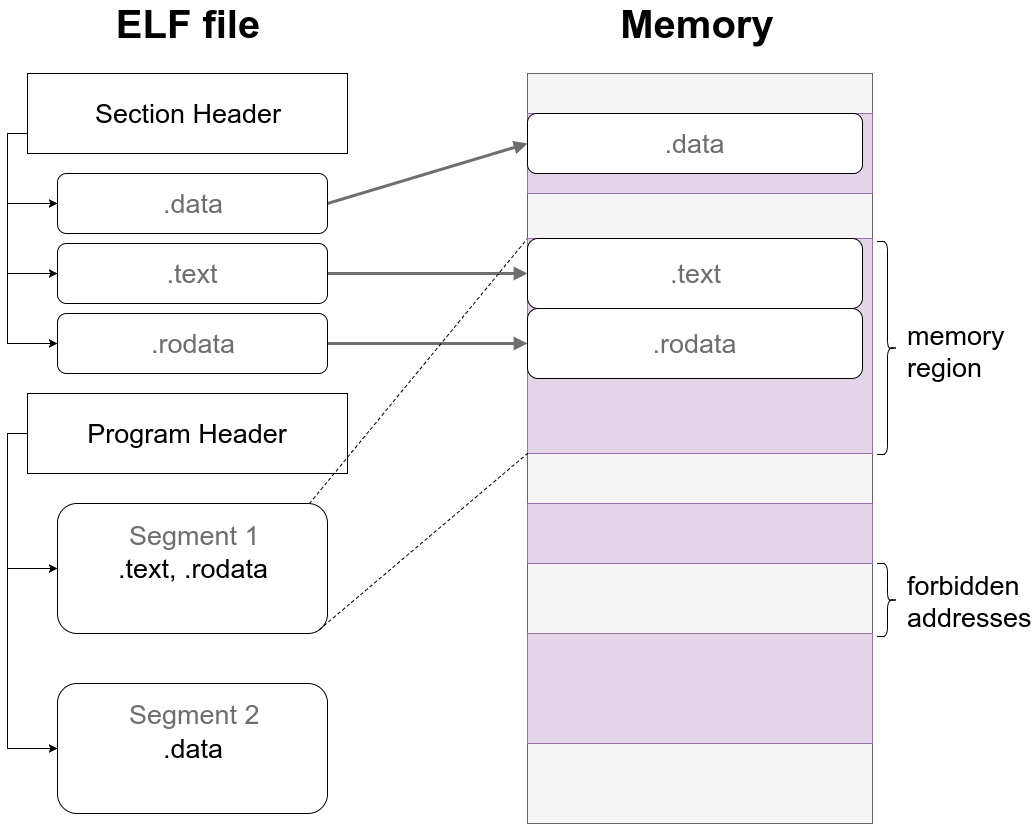
\includegraphics[scale=0.28]{images/segments-to-memory.png}
\end{frame}

\begin{frame}[fragile]{\subsecname}

\begin{shell}
> objdump -l symb
\end{shell}

{
\setlength{\tabcolsep}{5pt}
    \begin{tabular}{l l l l l l l}

        \textbf{Type}& \textbf{Offset} & \textbf{VirtAddr} & \textbf{FileSize} & \textbf{MemSize} & \textbf{Flags} & \textbf{Align}  \\\hline
        LOAD & 0    & 0x400000 & 0xc6 & 0xc6 & r-x & 0x200000 \\
        LOAD & 0xc8 & 0x6000c8 & 0x10 & 0x10 & rw- & 0x200000 \\

\hline
\end{tabular}
}

\begin{shell}
 Section to Segment mapping:
  Segment Sections...
   00     .text 
   01     .data 
\end{shell}

Loader uses flags to set up permissions in page tables.
\end{frame}


\begin{frame}[fragile]{With more sections}


\begin{asmexample}
global _start       

section .text        
  _start: jmp _start  
page 
section .data      
db 10

section .rodata
db 1

section .bss
resq 1024
\end{asmexample}

\end{frame}

\begin{frame}[fragile]{With more sections}

\begin{shell}
> objdump -l symb
\end{shell}

{
\setlength{\tabcolsep}{5pt}
    \begin{tabular}{l l l l l l l}

        \textbf{Type}& \textbf{Offset} & \textbf{VirtAddr} & \textbf{FileSize} & \textbf{MemSize} & \textbf{Flags} & \textbf{Align}  \\\hline
        LOAD & 0    & 0x400000 & 0xb8 & 0xb8 & r-x & 0x200000 \\
        LOAD & 0xb8 & 0x6000b8 & 0x01 & 0x2008 & rw- & 0x200000 \\

\hline
\end{tabular}
}

\begin{shell}
 Section to Segment mapping:
  Segment Sections...
   00     .text .rodata 
   01     .data .bss 
\end{shell}

\pause
    \begin{itemize}
        \item  .bss spares space in file
        \item  .rodata has execution permissions but it seems to be fine.
    \end{itemize} 
\end{frame}



\subsection{Static linking: summary}
\begin{frame}{\subsecname}

    {\usebeamerfont{title} Compiler }

    \begin{itemize}
        \item  Generates code with stubs for absolute addresses.
        \item  Generates symbol table.
        \item  Generates relocation tables for sections in need.
\end{itemize} 

    {\usebeamerfont{title} Static linker }
    \begin{itemize}
        \item Relocates pieces of code and data.
        \item Fills in stubs found in relocation tables.
        \item Creates program headers. 
    \end{itemize} 
\end{frame}

\subsection{Notes on C}

\begin{frame}{\subsecname}
    \begin{itemize}

        \item  All symbols are global by default.
        \item  \c{static} makes symbol local.
        \item  Long string literals and constants are likely to be in .rodata.
        \item  Zero initialized data in .bss (makes file smaller).
        
\end{itemize} 
\end{frame}



\section{Shared libraries}

\subsection{What are shared libraries?}

\begin{frame}{\subsecname}
    \begin{itemize}
        \item  Third type of ELF files.
        \item Separate file, after linking.
            \begin{itemize} 
                \item  \texttt{.dll}, \texttt{.so}
            \end{itemize} 
        \item Can be updated separately.
        \item Exposes some of global variables and functions.
        \item Relocation is partially performed.
        \item \textbf{Reusable by  other running processes}.
        \item  Spares memory, but has additional costs when using.
    \end{itemize}

    Executable files use many libraries.
\end{frame}

\begin{frame}{Relocations in a shared library}
    Kinds:
\begin{itemize}
    \item Links to locations in the same library (resolved by  static linker).
    \item Symbol dependencies (usually in the different object) -- performed by dynamic linker at runtime. 
\end{itemize} 

\end{frame}


\subsection{Dynamic linker}

\begin{frame}{Dynamic linker's job}

\begin{enumerate}
    \item Find and load dependencies. 
    \item Perform relocation. 
    \item Initialize the application and its dependencies 
    \item Pass the control to the application. 
\end{enumerate}
\end{frame}

\begin{frame}[fragile]{How to find which libraries we need?}
    \begin{itemize}
        \item  Search locations: 
    \begin{itemize}
             
        \item  rpath -- to be found in section .dynamic
         \item  \sh{LD_LIBRARY_PATH} environment variable.
         \item  runpath -- to be found in section .dynamic
         \item  List in the file /etc/ld.so.conf. 
         \item  Standards such as \texttt{/lib} 
    \end{itemize}    
        \item  Depth-first-search order, dependencies and their dependencies.
        \item  Remember, there is an order on dependencies!
        \item  Does not load the same library twice.
    \end{itemize} 
\end{frame}



\begin{frame}{How to select a symbol?}

    As in static linking, we search by name through the symbol tables.

    Symbol can be defined in multiple objects, only one will exist in runtime.

    Depending on a set of existing objects, its location may change.
    
    \textbf{Lookup scope of an object file} an ordered list of a subset of the loaded objects.

\end{frame}


\begin{frame}{Lookup scopes}
    Last to first priority.

        \begin{itemize}
    \item  Global: the executable and all its dependencies recursively,
        in a \emph{breadth-first search} order.

                Starts with the executable.
    \item  Legacy: look in metadata if \sh{DF_SYMBOLIC} flag is set.
        If yes, local definitions are preferred.

    \item Everything opened by \c{dlopen} call have a common additional separated scope. Not searched for normal lookups.
 
    \end{itemize} 
    
    \sh{LD_PRELOAD} allows to add a library to global scope right after the executable itself.

\end{frame}
\subsection{Position Independent Code}

\begin{frame}{How to perform relocations?}
    \begin{itemize}
        \item  Relocations in runtime lead to patching addresses.
        \item  Modified pages can not be shared, hence the advantages of 
            shared libraries pale.
    \end{itemize} 
        Can we write in a manner we can execute the code no matter the loading address?
    \end{frame}


\begin{frame}{Sharing library between processes}
    \begin{itemize}
 \item  .data and .bss  can not be shared anyway (each process should have its own global variables).
 \item  .text can be shared if consists of \textbf{position independent code (PIC)}.
 \item  .rodata can be shared if it has no relocations (e.g. an address of a variable).
\end{itemize} 

\end{frame}

\begin{frame}{RIP-relative addressing}
    RIP -- register holding the address of current instruction (Program Counter)

    Intel 64 supports RIP-relative addressing out-of-the-box. 

    Can we just change all addressing to RIP-relative? 
    \begin{itemize}
         \item  Works for addresses of \emph{local} variables and functions: we
             know the offsets between current position in code and everything
             from the same object file.

         \item  \textbf{Not for exported or imported symbols}: we do not know which object will provide them.

    \end{itemize} 

    Solution: add level of indirection using \textbf{Global Offset Table}.
    %FIXME illustration?
\end{frame}


\subsection{Global Offset Table}

\begin{frame}{\subsecname}

    \begin{itemize}
        \item A table storing addresses of global variables and functions.
        \item Unique per object file. 
        \item  Dynamic linker fills it with correct addresses.
\end{itemize}

\end{frame}
\begin{frame}[fragile]{\subsecname}
    \begin{tabular}{l l}
    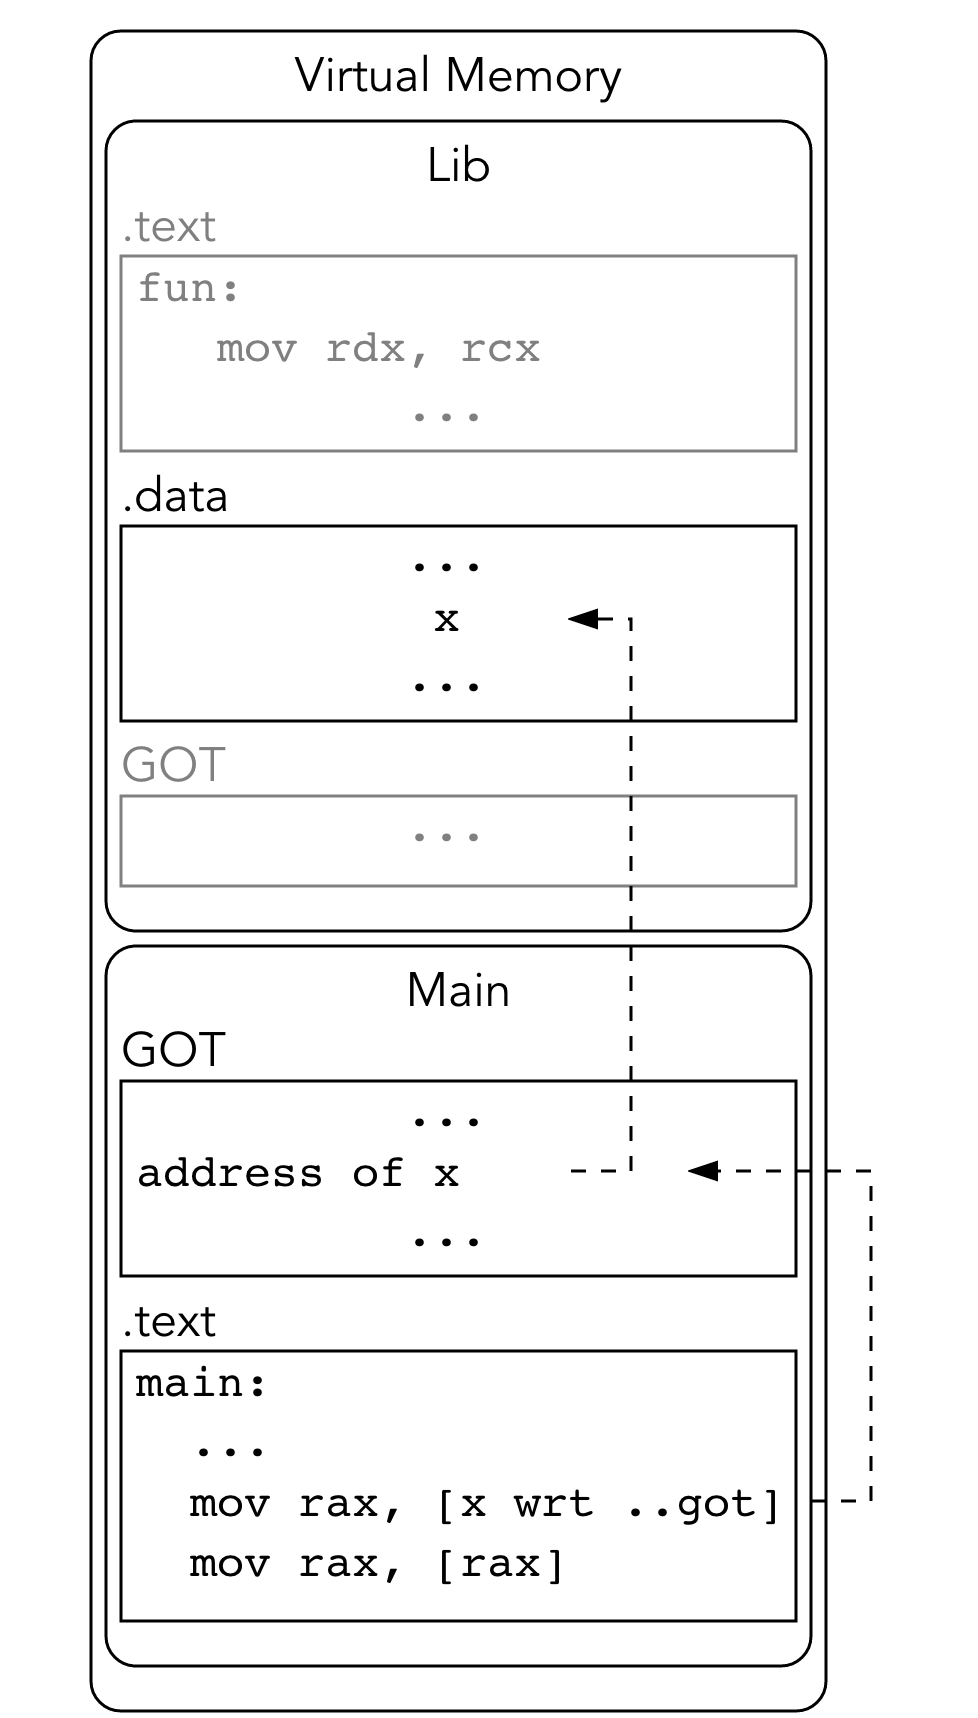
\includegraphics[height=0.9\textheight]{images/got.png} 
    &
        {Accessing a global variable \texttt{x} }
    
    \end{tabular}
\end{frame}


\begin{frame}{Coding time}
        NASM uses the \asm{rel} keyword to achieve \asm{rip}-relative
        addressing. This does not involve GOT nor PLT. 
    \begin{itemize} 
        \item  Minimal assembly example.  
        \item  Note a problem with hardcoded linker name.
        \item  Using \texttt{ldd}
\end{itemize} 
\end{frame}

\begin{frame}{Types of relocations}
   All are processor-specific.

    Tells how specifically should we alter an instruction operand.
    
    \sh{R_X86_64_64} for ``replace with immediate address'', but others are 
    more complex.

\end{frame}


\subsection{Procedure Linkage Table}


\begin{frame}{\subsecname}

    Calling globally available procedures is based on an augmented GOT.

    There are many procedures exported, few used. 

    We do not want the linker to resolve them until needed.

    So, implement a lazy binding using \textbf{Procedure Linkage Table}
\end{frame}



\begin{frame}{\subsecname{} -- before resolving}
    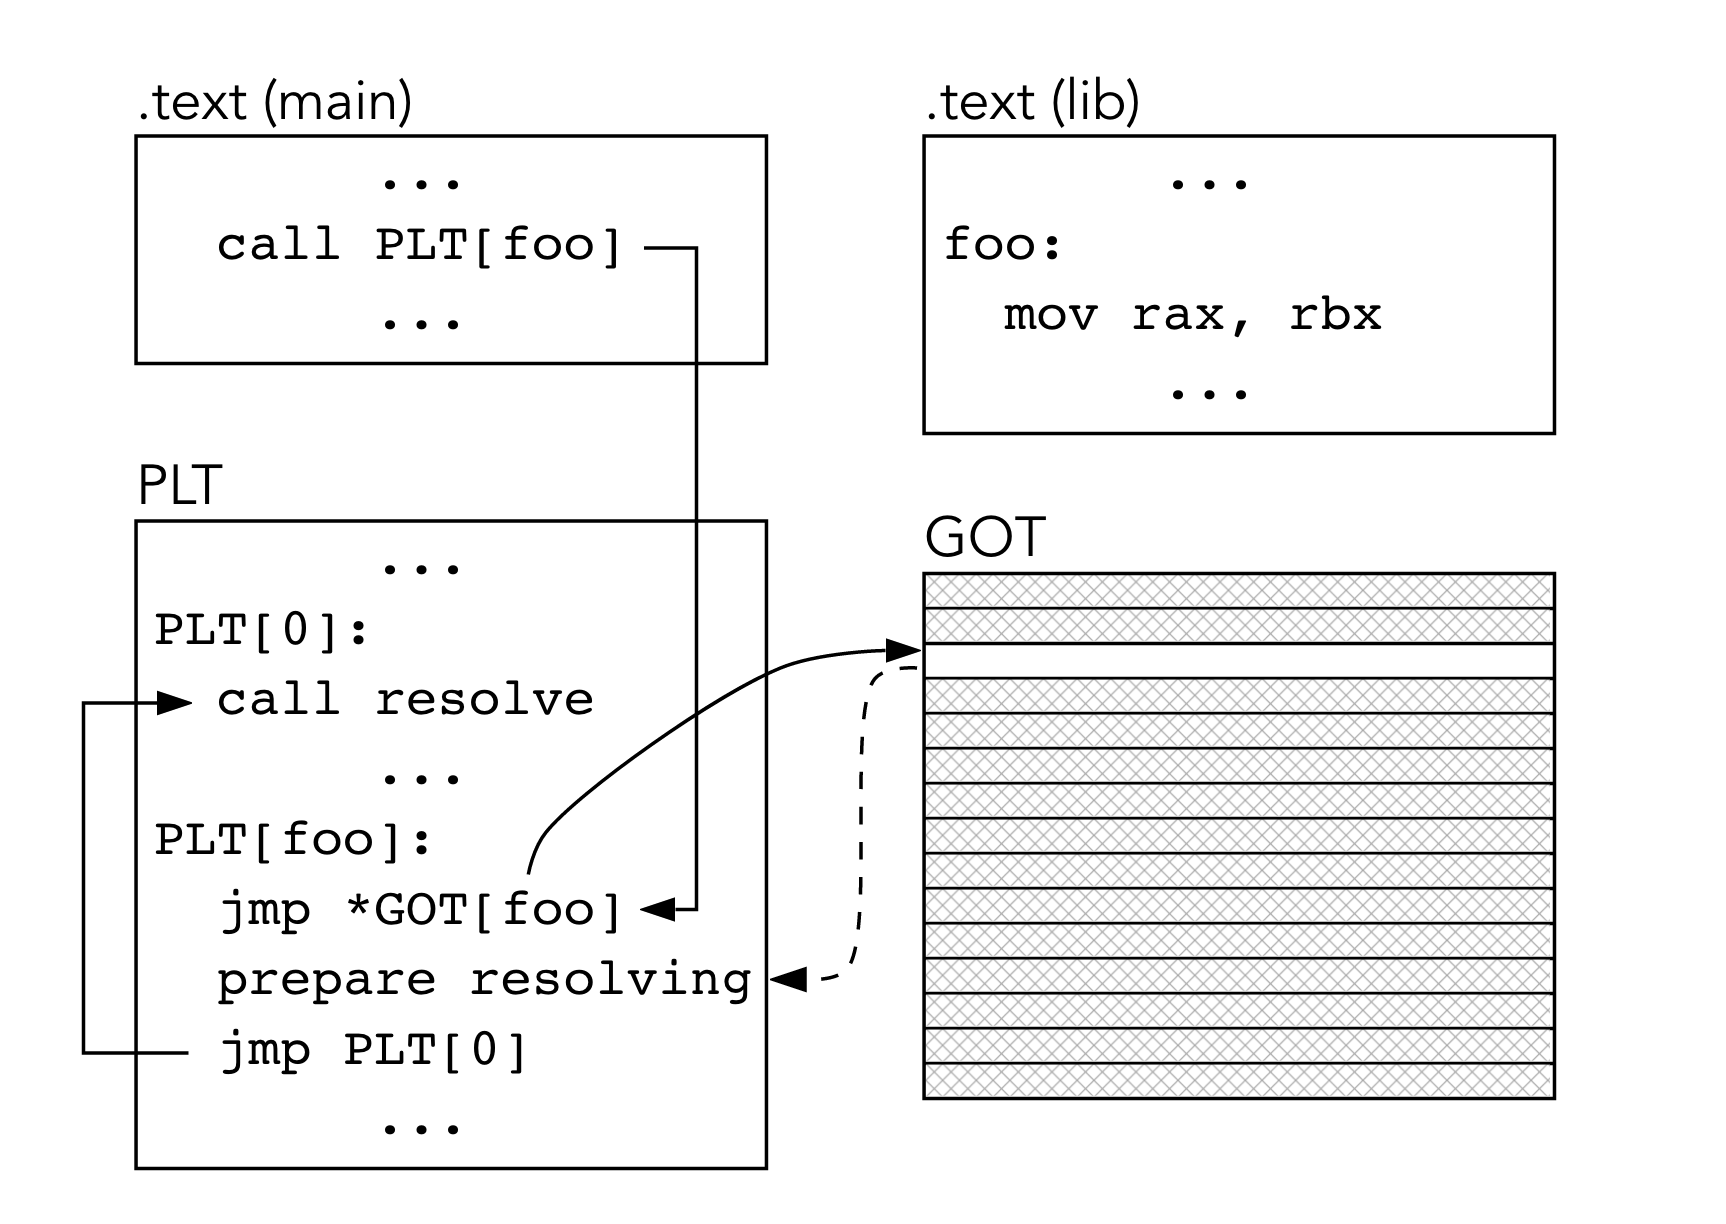
\includegraphics[height=0.9\textheight]{images/plt-before.png} 
\end{frame}

\begin{frame}{\subsecname{} -- after resolving}
    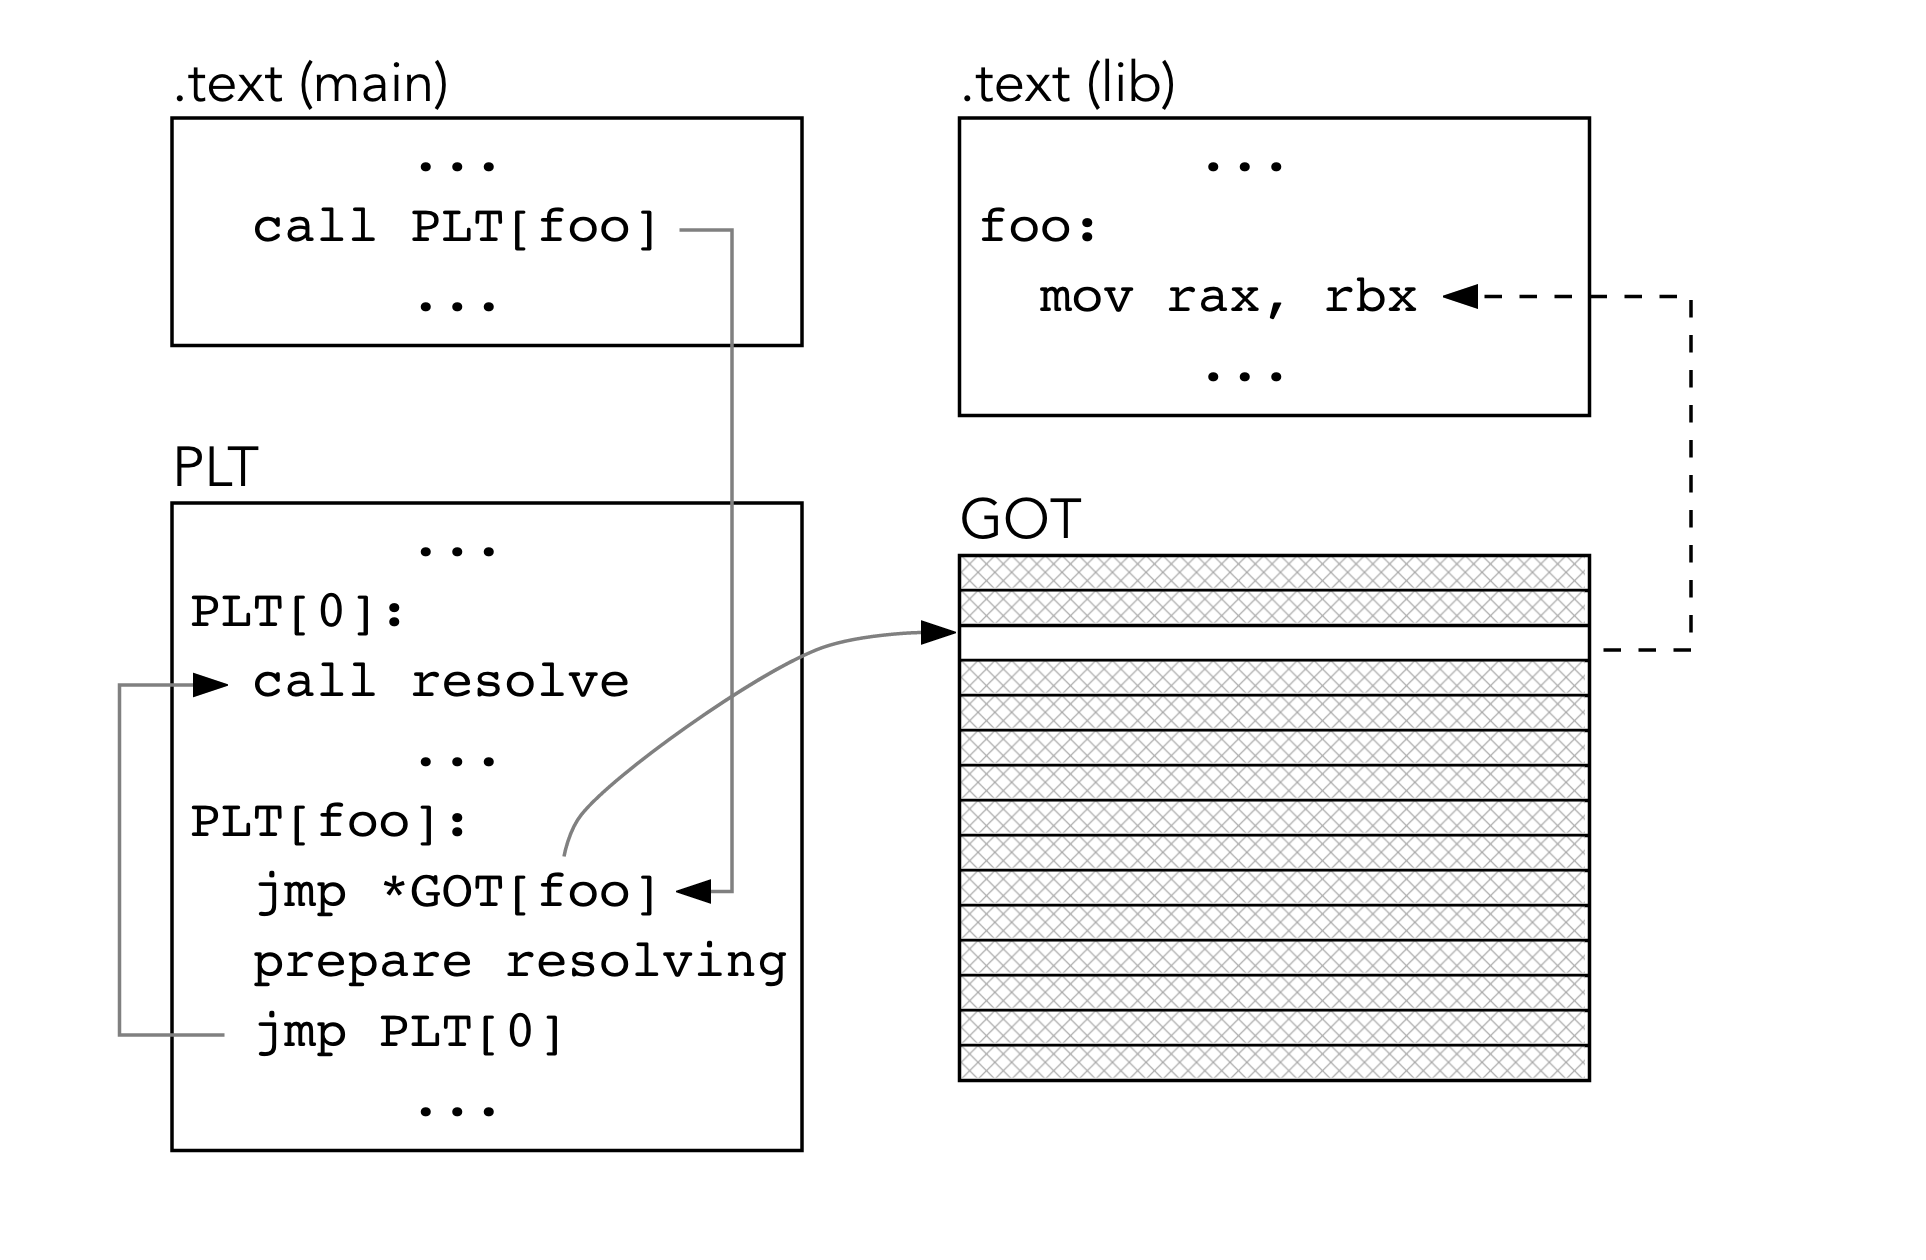
\includegraphics[height=0.9\textheight]{images/plt-after.png} 
\end{frame}


\subsection{Symbol addressing summary}

\begin{frame}{\subsecname}
    \begin{itemize}
        \item  Writing and exploring a shared library in C.
        \item  Writing and exploring a shared library in Assembly.
    \end{itemize} 
\end{frame}


\begin{frame}{\subsecname}
Assuming the main executable file is not PIC.

The symbol can be:

\begin{enumerate}
    \item Defined in executable and used locally there -- trivial.
        
    \item Defined in dynamic library and unavailable to external objects.

        In presence of PIC, it is done by using \asm{rip}-relative addressing
        (for data) or relative offsets (for function calls). 

    \item Defined in executable and used globally.
        
        Requires  GOT/PLT  if the caller is external. 

    \item Defined in dynamic library and used globally.

        Requires GOT/PLT.
\end{enumerate} 

\end{frame}


\subsection{Visibility}
\begin{frame}
Kinds of visibility: local, static, global to exec, global to process
\end{frame}

\begin{frame}
How to mark as public?
\end{frame}

\begin{frame}
HIDE SYMBOLS BY DEFAULT (drep 18)
\end{frame}


\begin{frame}
    EXPORT MAPS (drep 22)
\end{frame}

\section{Optimization}

\begin{frame}{\subsecname}
    Performance boosters already inside ELF files.

    \begin{itemize}
        \item Hash map: symbols $\mapsto$ addresses.

        \item Bloom filter (does this object file define a symbol $x$?).
    \end{itemize} 
    %FIXME illustrate with READELF
\end{frame}


\begin{frame}
GO WITH THE SECTION P.286
\end{frame}



\begin{frame}
DSO CONSTRUCTORS AND DESTRUCTORS: HOW TO MAKE, IMPACT
\end{frame}

\begin{frame}
    CHECK DREPPER's WORK : PAGE 13 
\end{frame}

\begin{frame}
    CHECK DREPPER's WORK : PAGE 26, names
\end{frame}

\begin{frame}
    \c{const char[] or const char*}

\end{frame}



\begin{frame}
ARRAYS OF FUNCTION POINTERS
\end{frame}

\section{Overriding symbols}

\subsection{Using \texttt{LD\_PRELOAD}}


\begin{frame}{\subsecname}
    
   \texttt{LD\_PRELOAD} is an environment variable.

    Stores path to libraries to load before anything else. 

    These have the highest priority.
\end{frame}


\begin{frame}{Example: overriding glibc functions}
    \texttt{glibc} is usually dynamically linked.

    Let us override a function!

\end{frame}


\section{Code models}
\subsection{What is  a code model}

\begin{frame}[fragile]{\subsecname}
    In our case, \textbf{code model} is a mode of generating instructions related to addressing.

    RIP-relative addresses are limited by offsets of 32 bits. What if we need more?

    Usually it is enough; no need to waste more bytes clogging the instruction cache.

    Otherwise we use multiple instructions, like:

\begin{asmexample}
    mov rax, 0x12345
    mov rcx, [rax]
\end{asmexample}

    gcc option: \sh{ -mcmodel=small/medium/large}
\end{frame}

\subsection{Six models}

\begin{frame}

Besides kernel-related, there are six code models:

    \begin{itemize}

        \item  PIC or Non-PIC modifier;
            \begin{itemize}
 
        \item  Small -- what we are used to
        \item  Large -- all offsets are now 64 bit, performance is hit.
        \item  Medium -- like small, but selected huge arrays are addressed like in large.
        \end{itemize} 
\end{itemize} 

    Examples follow.
\end{frame}





%\begin{frame}[allowframebreaks]
%\frametitle{References}
%\bibliography{biblio} 
%\end{frame}


\iffalse
Litterature:
my book
ABI
Ulrich drepper
\fi
\end{document}


\iffalse
\begin{frame}[fragile]{Sections -- before linking}
    \begin{shell}
> readelf -S symb.o
    \end{shell}

{\small
\setlength{\parindent}{-0.5cm}
\setlength{\tabcolsep}{3pt}
\begin{tabular}{l l l l l l l l l l }
\textbf{Name}& \textbf{Type} & \textbf{Address} & \textbf{Offset} & \textbf{Size}& \textbf{EntSize} & \textbf{Flags} & \textbf{Link} & \textbf{Info} & \textbf{Align} \\
.data & PROGBITS   & 0 & 240  & 10 & 0 & WA & 0 & 0 & 4 \\
.text & PROGBITS   & 0 & 250  & 16 & 0 & AX & 0 & 0 & 16 \\
.shstrtab & STRTAB & 0 & 270  & 3d & 0 & 0  & 0 & 0 & 1  \\
.symtab   & SYMTAB & 0 & 2b   & c0 & 18& 0  & 5 & 6 & 4  \\
.strtab   & STRTAB & 0 & 370  & 2d & 0 & 0  & 0 & 0 & 1  \\
.rela.data& RELA   & 0 & 3a0  & 18 & 18& 0  & 4 & 1 & 4 \\
.rela.text& RELA   & 0 & 3c0  & 30 & 18& 0  & 4 & 2 & 4 \\

\end{tabular}
}
\pause
    \begin{itemize}
        \item  All addresses are 0
    \end{itemize}
\end{frame}

\fi

